\begin{frame}[c]\label{a.1}
\frametitle{Supercooled Liquids a Glance}%: Why Study Supercooled Liquids?}%at is a Supercooled Liquid?}
\vspace{-12.0pt}
\begin{overprint}
\onslide<1-5>\begin{block}{\large \centering Why Study Supercooled Liquids?}
\vspace{6pt}
\centering A supercooled liquid contradicts our intuition on how \only<2->{slow (\textbf{glassy}) }dynamics relates to structure.
\end{block}
%\vspace{-4pt}}
\onslide<6->
\begin{block}{\large \centering Central Question}
\vspace{6pt}
\centering How to understand the dramatic slowdown and dynamical heterogeneity of supercooled liquids?
\end{block}
\end{overprint}
%
%\vspace{4pt}
\begin{columns}
\begin{column}{0.5\textwidth}
\centering  \uncover<2->{\textbf{\large Dynamics}}

\begin{figure}[t]

\begin{overprint}
\onslide<2>\centering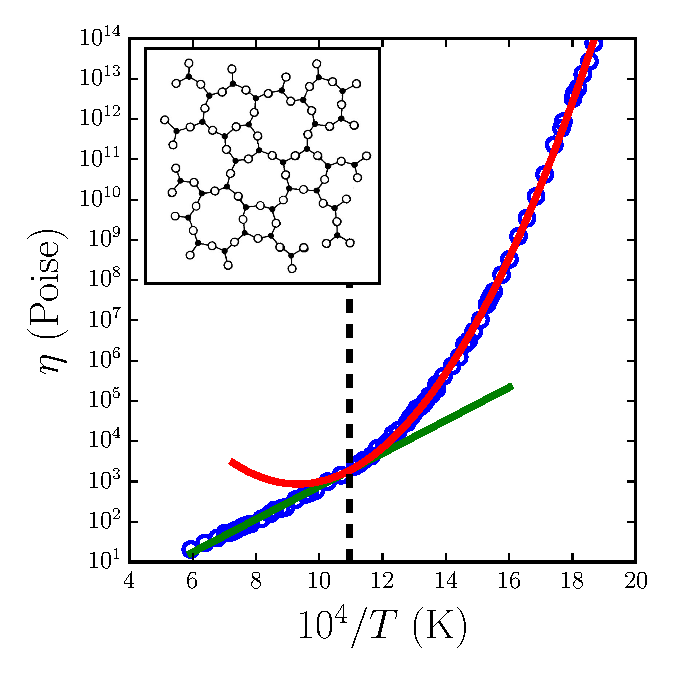
\includegraphics[height=0.6\textheight]{intro_glassy/timerelax_b2o3_4.pdf}
\caption{Viscosity of boron oxide ($\mathrm{B_2 O_3}$) (Tweer, Simmons, and Macedo, \textit{J. Chem. Phys.},  1970).}

\onslide<3>\centering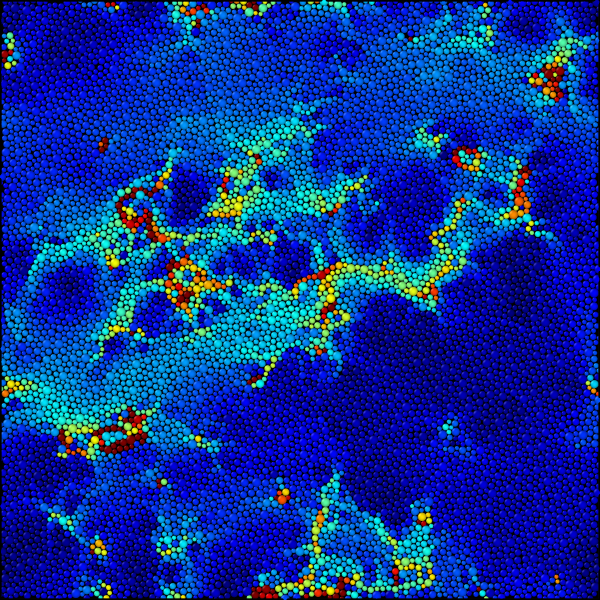
\includegraphics[height=0.6\textheight]{intro_glassy/softspots_280.png}
\caption{\textbf{Dynamical heterogeneity}: localized mobile regions (at early times) that spread over time.}  

\onslide<4->\centering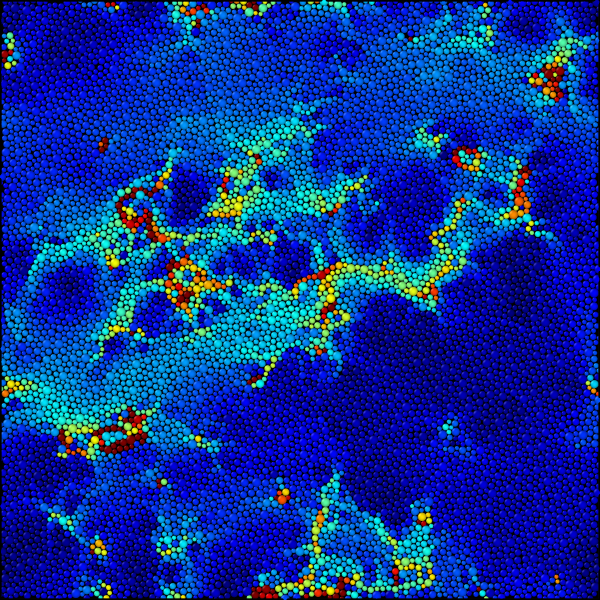
\includegraphics[height=0.6\textheight]{intro_glassy/softspots_280.png}
\caption{\textbf{Dynamical heterogeneity}: localized mobile regions (at early times) that spread over time.}  
\end{overprint}

\end{figure}



% \only<4->
% {
% \begin{figure}[t]
% \centering
% \includegraphics[height=0.6\textheight]{figures/timerelax_poly12_1.pdf}
% \caption{\textbf{Super-Arrhenius: }Dramatic slowdown at temperatures $T$ below onset temperature $T_\mathrm{o}$ (dashed line).}
% \end{figure}
% }

% \only<7->{
% \begin{figure}[t]
% \includegraphics[height=0.73\textheight]{figures/facilitation.png}
% \caption{2D 50:50 Binary Lennard-Jones system, showing the coordinated movement of particles (Keys et.al. 1, 021013, \textit{Phys. Rev. X}, 2011).} 
% \end{figure}
% }

\end{column}

\begin{column}{0.5\textwidth}
\centering  \uncover<5->{\textbf{\large Structure}}


\begin{figure}[t]
\begin{overprint}
\onslide<5>\centering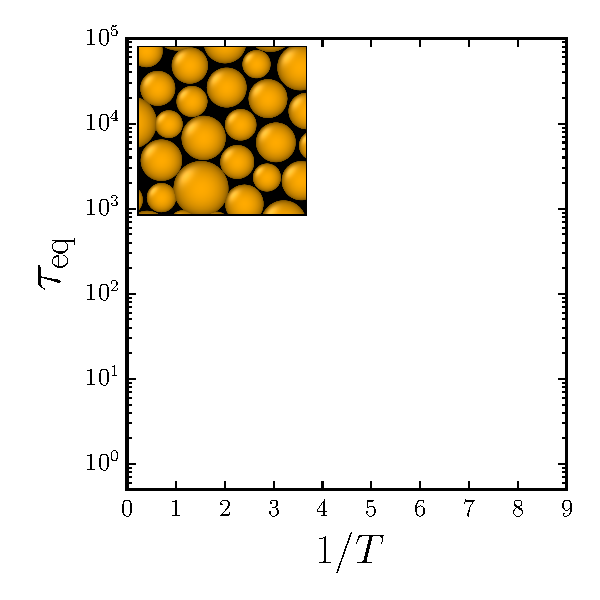
\includegraphics[height=0.6\textheight]{intro_glassy/timerelax_poly12_0.pdf}\caption{It is not obvious from the structure where the heterogeneity is coming from!}
\onslide<6->\centering\includegraphics[height=0.6\textheight]{intro_glassy/timerelax_poly12_1.pdf}
\caption{Radial distribution function (RDF). Data sweeps across \textbf{4 decades in relaxation time}.}

% (it is disordered and well-dispersed)!}% structure of supercooled liquids is disordered and homogeneous at all temperatures}
\end{overprint}

%Locations of the peaks in the radial distribution function (RDF) remains the same, despite dramatic slowdown in dynamics.}
\end{figure}


% \only<6->{
% \begin{figure}[t]
% \centering
% \uncover<7->{\includegraphics[height=0.6\textheight]{figures/gr_poly12_single.pdf}}
% \caption{Local structure (from the RDF) remains qualitatively same under a wide range of supercooled conditions.}
% \end{figure}
% }

\end{column}
\end{columns}
\end{frame} 